\chapter{Results}
\label{ch:results}
%
% The scope of this thesis includes the generation, animation and rendering of the
% surface of an open ocean in real-time. We focus our interest on the synthesis of
% animated ocean surface geometry, for which we will adopt a set of models from
% oceanographic research.

The previous chapter discussed in detail the approach we took to synthesize
the animated ocean surface, including, one, a number of optimizations to reduce
the computational workload, and, two, a level of detail mechanism which does
not only give us fine-grained control over model detail, but also allows us to
reduce potential tiling artifacts. In addition, we gave an overview of our demo
application, which integrates our approach to ocean surface synthesis
with real-time rendering algorithms tailored specifically for display of
the open ocean.
Thus, with our demo application at hand, we may move on to discuss the
actual results we were able to achieve.

The remainder of this chapter is organized as follows:
Section \ref{sec:results:fft} gives a compact overview of the performance
improvements which we were able to attain for the \InvFourierTransform.
Section \ref{sec:results:synthesis} delineates the pitfalls we encountered
in the context of ocean surface synthesis with wave spectra, and what measures
we took to either overcome or sidestep them.
Last, Section \ref{sec:results:fidelity} discusses the level of visual fidelity
we were able to obtain, with focus on the different wave spectra, as well as
our level of detail approach.

% Before we delve into details, one may look at Figure~\ref{fig:results} which
% depicts all componenents which are part of our ocean lighting implementation.
% compare lighting of all spectrum types (same parameters)

\section{Fourier Transform}
\label{sec:results:fft}
We did not reproduce the current state of art with regard to the \FourierTransform,
i.e. compute the \IDFT on the GPU (GPGPU, CUDA, clfft). The reasons are varying,
but the most compelling is debugging. We have found it difficult to make sure
that the spectrum is synthesized correctly, because it is essentially gaussian noise,
thus deviations caused by a faulty implementation still lead to results which hold
up to casual scrutiny. Thus, keeping all spectrum related computation on the
CPU side allowed us to assert corretness more easily.
As we already did a MATLAB implementation and a native one
in ObjC, an additional one would have expanded the scope of this work unreasonably.
Still, FFTW does an acceptable job performancewise. Note, that we employed the
float precision variant of FFTW, since it has proven to provide sufficient
numerical accuracy for our use case, and outperforms the double precision variant
by a factor of 1.5.

Simple \InvFourierTransform vs \InvFourierTransform of two hermitian spectra
Pattern synthesis at full resolution for all datasets
Pattern synthesis with our multi-resolution approach

\section{Pattern Synthesis}
\label{sec:results:synthesis}
Although all spectrum types give convincing results geometry-wise, it is the
Preetham spectrum and the Unified spectrum that work best with the lighting
algorithm by \cite{article:oceanlighting}. Probable cause is that the JONSWAP
spectrum and the Donelan spectrum give not that good an approximation of the
ocean surface's mean square slope (\ref{app:mss}). The mean square slope is a
core component of the lighting model by \cite{article:oceanlighting}, and thus
has large influence on the result.

In the beginning we needed several fudge factors to generate acceptable results,
specifically, we were always required to add some scaling factor in the XZ plane
or in the Y direction. And the fudge factors needed to change if spectrum
parameters changed.
Only after implementing correct integral domain conversion for the different
spectra did we obtain consistent results across all spectrum models. It made all
the difference, since now we get consistent, believable as well as
comprehensible results for all spectra. No fudge factors are required anymore,
everything works out of the box.

\section{Visual Fidelity}
\label{sec:results:fidelity}
%
\begin{figure}
\centering
 \subtop[Sun Contribution]
 {
  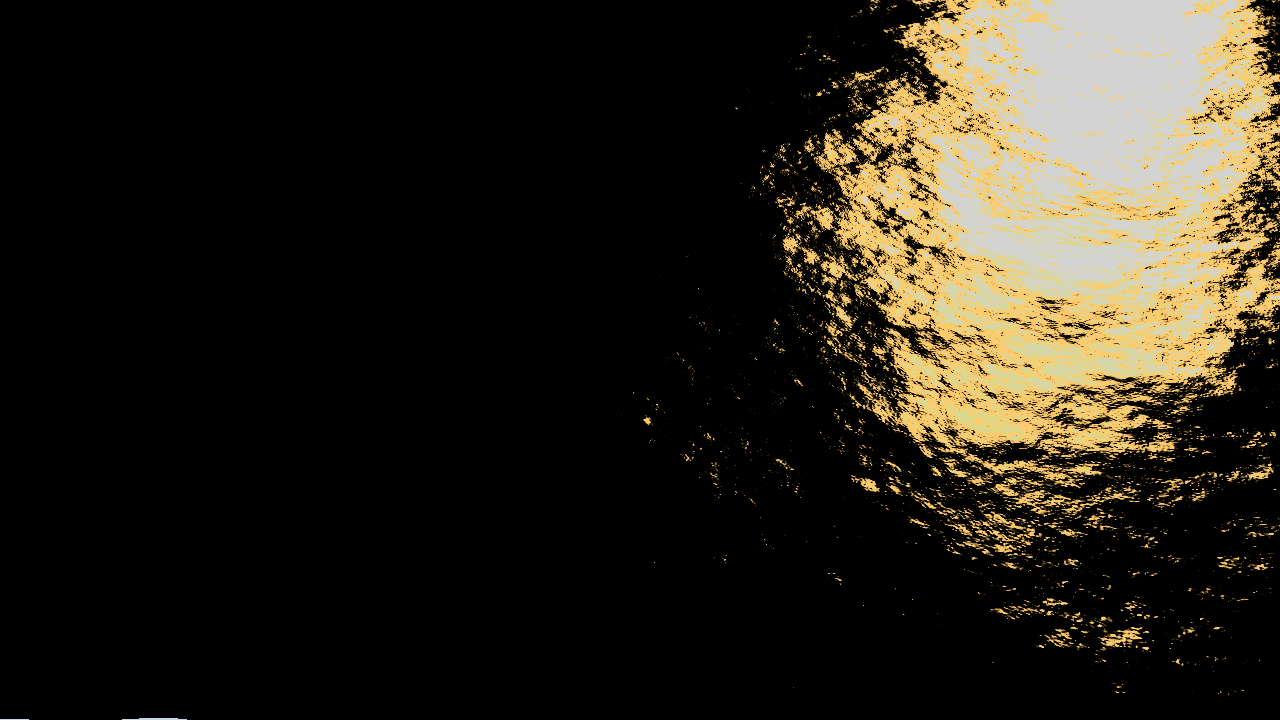
\includegraphics[width=0.48\textwidth]{figures/31-07-2017_10-47-08_ross.png}
	\label{fig:results:ross}
 }
 \hfill
 \subtop[Sky Contribution]
 {
  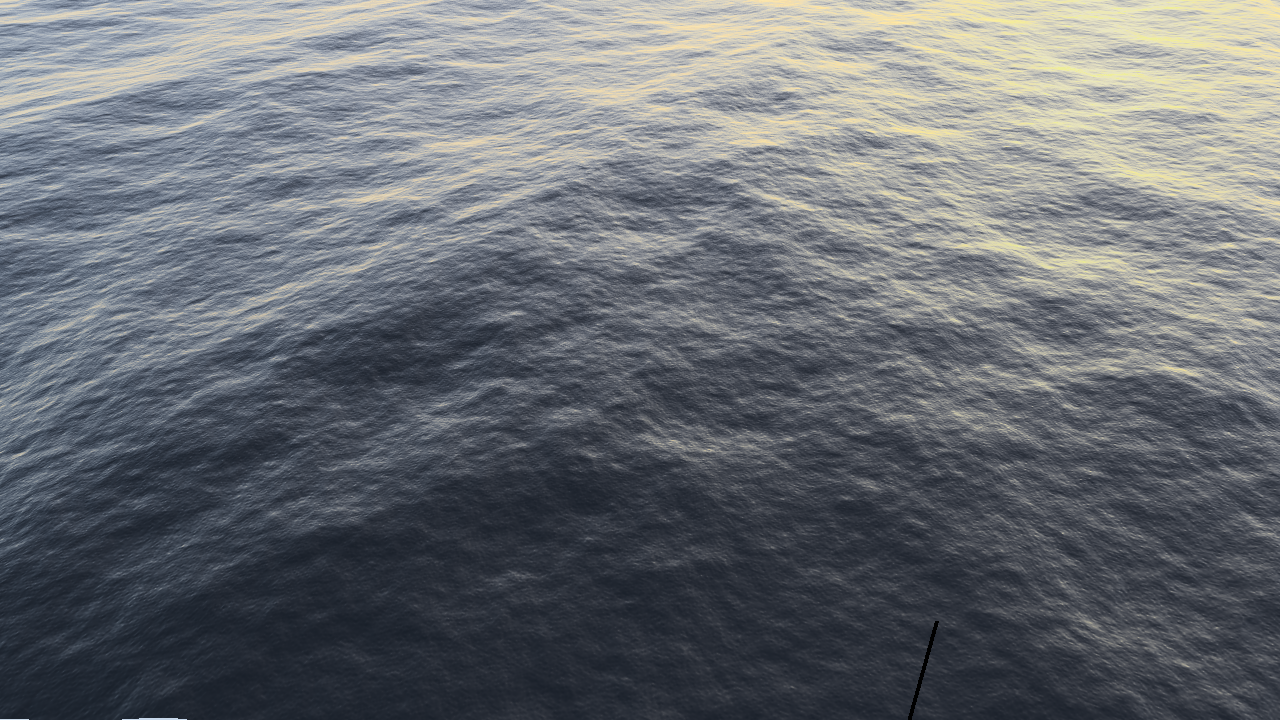
\includegraphics[width=0.48\textwidth]{figures/31-07-2017_10-47-08_sky.png}
	\label{fig:results:sky}
 }
 \hfill
 \subtop[Sea Contribution]
 {
  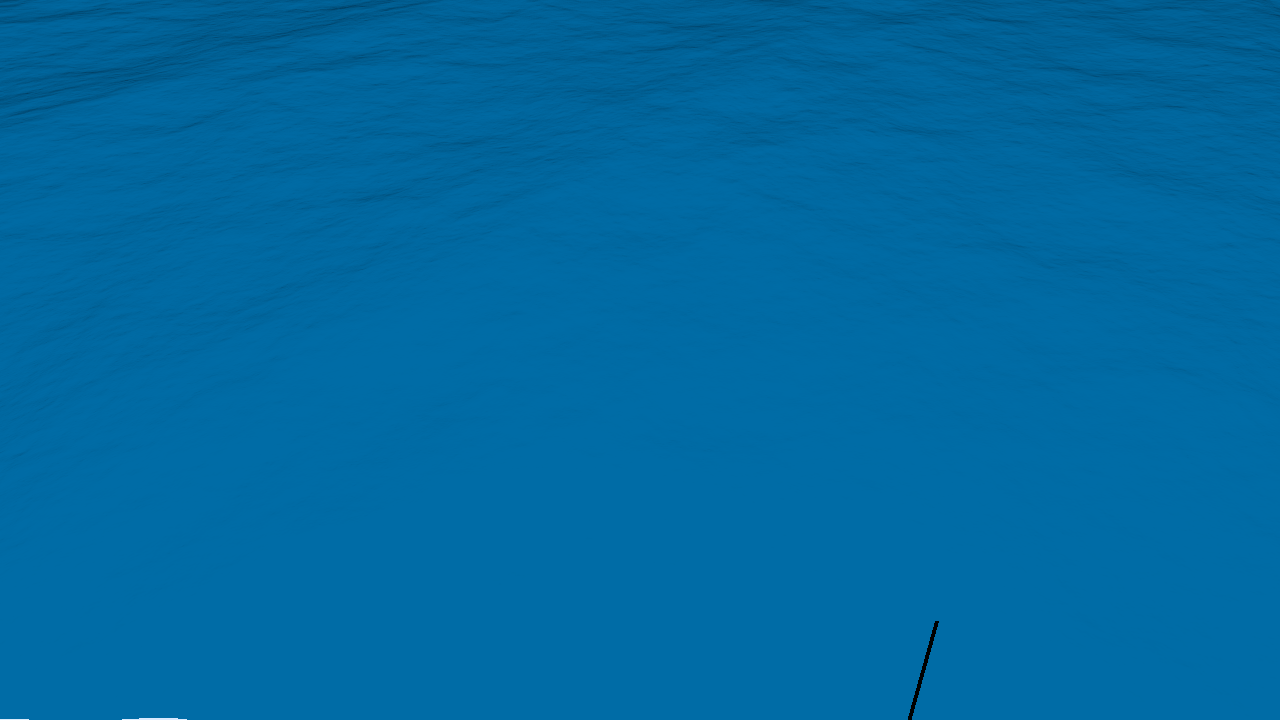
\includegraphics[width=0.48\textwidth]{figures/31-07-2017_10-47-08_sea.png}
	\label{fig:results:sea}
 }
 \hfill
 \subtop[Whitecaps Contribution]
 {
  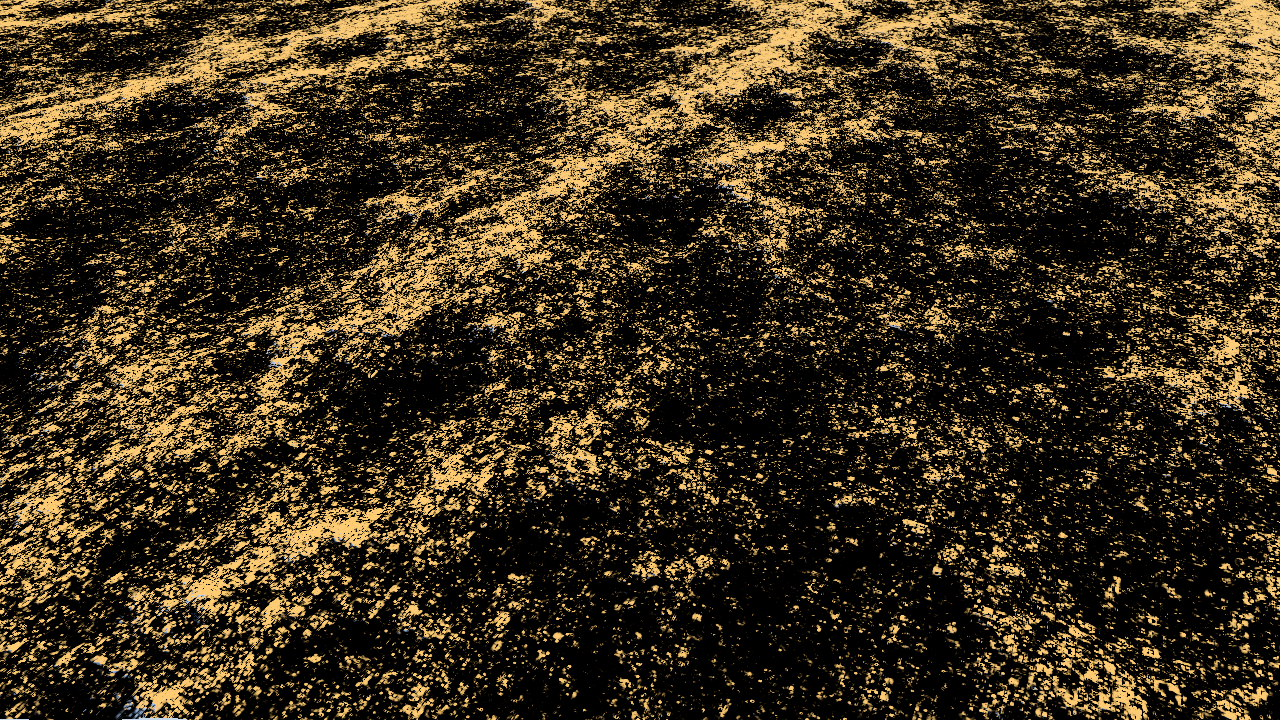
\includegraphics[width=0.48\textwidth]{figures/31-07-2017_10-47-08_whitecaps.png}
	\label{fig:results:whitecaps}
 }
 \hfill
 \subtop[Final Result]
 {
  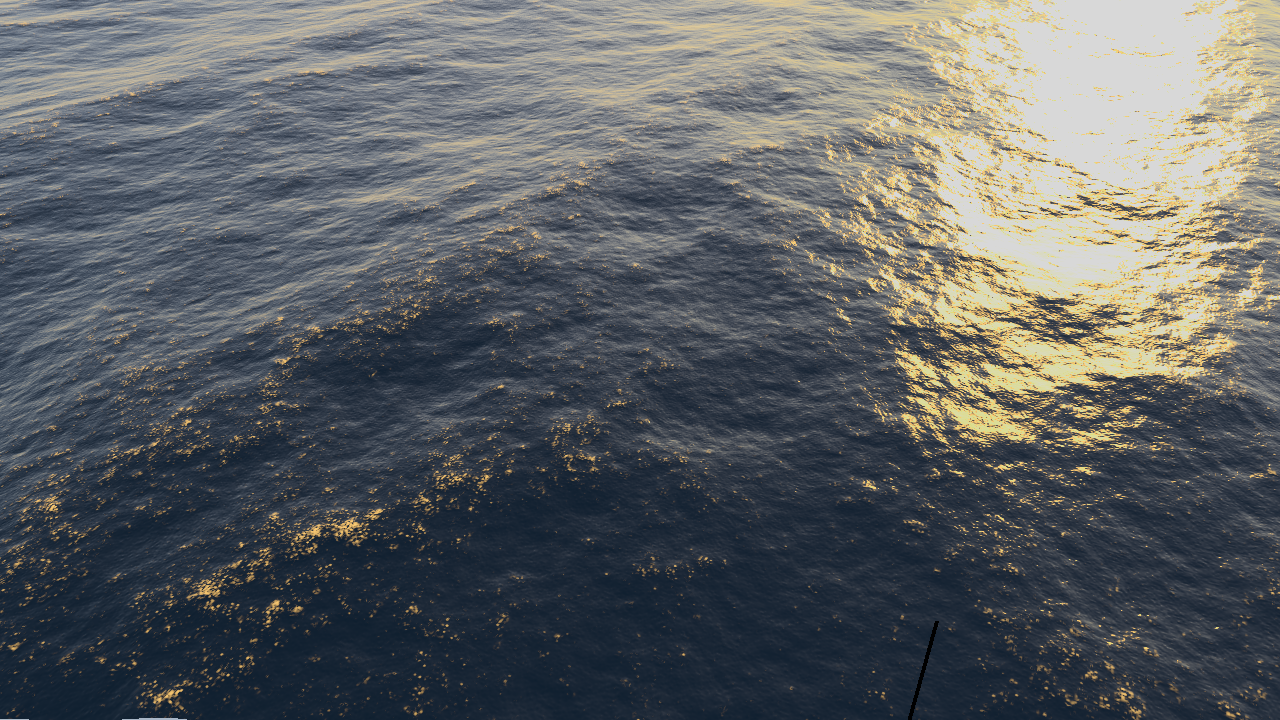
\includegraphics[width=\textwidth]{figures/31-07-2017_10-47-08_complete.png}
	\label{fig:results:complete}
 }
\caption{An overview of all ocean lighting terms involved in our implementation
of \citet{article:oceanlighting,misc:oceanlightingfft} and \citet{article:whitecaps}.
\subcaptionref{fig:results:ross} Sun light reflected by the water surface.
\subcaptionref{fig:results:sky} Sky light reflected by the water surface.
\subcaptionref{fig:results:sea} Light refracted from the water body.
\subcaptionref{fig:results:whitecaps} Whitecap foam.
\subcaptionref{fig:results:complete} All previous terms combined into the final
result.
}
\label{fig:results}
\end{figure}
%
Images of all partial terms involved in ocean lighting (specular by sun,
reflection of sky, refracted light, whitecaps)

Troubles with reflection vectors below horizon
Troubles with bright patches caused by reflection
Troubles with dark patches caused by reflection
Troubles with sundisk (XYZ to sRGB)

Tiling images

Comparison full resolution patterns vs multi-resolution scheme

Maybe different tonemapping settings